\documentclass{ujarticle}
\usepackage{moreverb}
\usepackage{amsmath}
\usepackage[dvipdfmx]{graphicx}
\title{熱伝導方程式の差分法による解法}
\begin{document}
\maketitle
\section{目的}
湯気のシミュレーションにおいて熱伝導方程式を解く必要がある。
熱伝導方程式の差分法による解法をまとめる。
\section{熱伝導方程式}
一次元の熱伝導方程式は次式で表される。
\begin{equation}
\frac{\partial T}{\partial t} = \alpha \frac{\partial^2T}{\partial^2x}
\end{equation}
$T$は温度、$\alpha$は温度伝導率であり、次式より求まる。
\begin{equation}
\alpha=\frac{\lambda}{\rho c_{p}}
\end{equation}
$\lambda$は熱伝導率、$\rho$は密度、$c_{p}$は定圧比熱である。
\section{偏導関数の近似}
差分法では偏導関数を前進差分、後退差分で次のように近似する。
\begin{equation}
\frac{\partial f}{\partial x}=\frac{f_{i+1}-f_{i}}{\Delta x}
\end{equation}
\begin{equation}
\frac{\partial f}{\partial x}=\frac{f_{i}-f_{i-1}}{\Delta x}
\end{equation}
2階の偏導関数は1階の偏導関数であるから前進差分と後退差分を用いれば次式を得られる。
\begin{equation}
\frac{\partial^2 f}{\partial^2 x} = \frac{f_{i+1}-2f_{i}+f_{i-1}}{\Delta x^2}
\end{equation}
\section{陽解法}
前進差分を用いて数値解を求める方法は陽解法と呼ばれる。
$T_{x,t}$として陽解法による差分近似式は次式になる。
\begin{equation}
\label{t_diff}
\frac{T_{i,j+1} - T_{i,j}}{\Delta t} = \alpha\frac{T_{i+1,j}-2T_{i,j}+T_{i-1,j}}{\Delta x^2}
	\end{equation}
$T_{i,j+1}$について解くと次式になる。ここで$\gamma$は$\frac{\Delta t}{\Delta x^2}$となる。
\begin{equation}
T_{i,j+1}=\alpha \gamma T_{i+1,j} + (1-2 \alpha \gamma)T_{i,j}+\alpha \gamma T_{i-1,j}
\end{equation}

\section{陰解法}
後退差分を用いて数値解を求める方法は陰解法と呼ばれる。
差分近似式は次式となる。
\begin{equation}
\frac{T_{i,j+1}-T_{i,j}}{\Delta t} = \alpha \frac{T_{i+1,j+1}-2T_{i,j+1}+T_{i-1,j+1}}{\Delta x^2}
\end{equation}
これを整理すると次式になる。
\begin{equation}
-\alpha \gamma T_{i+1,j+1}+(1+2 \alpha \gamma)T_{i,j+1} - \alpha \gamma T_{i-1,j+1} = T_{i,j}
\end{equation}
陽解法とは異なり$T_{i,j}$から、次の時刻での$T_{i-1,j+1},T_{i,j+1},T_{i+1,j+1}$の3点を求める。
前式を行列で表すと次の式のようになる。

\[
  \left(
    \begin{array}{ccccc}
      1+2 \alpha \gamma & -\alpha \gamma  & 0 & \ldots & 0 \\
      -\alpha \gamma  & 1+2 \alpha \gamma & -\alpha \gamma & \ldots & 0 \\
       & \vdots &  & \ddots & \vdots \\
      0 & \ldots & -\alpha \gamma  & 1+2 \alpha \gamma & -\alpha \gamma \\
      0 & \ldots & 0 &  -\alpha \gamma  & 1+2 \alpha \gamma
    \end{array}
  \right)
  \left(
  	\begin{array}{c}
  		T_{1,j+1} \\ T_{2,j+1} \\ \vdots \\ T_{M-1,j+1} \\ T_{M,j+1} 
  	\end{array}
  \right)
  =
  \left(
  	\begin{array}{c}
 		T_{1,j} \\ T_{2,j} \\ \vdots \\ T_{M-1,j} \\ T_{M,j} 
  	\end{array}
  \right)
\]

前式の連立一次方程式を数値解法によって解く。このとき行列の$T_{i,j+1}$と$T_{M,j+1}$には境界条件を設定する。

\section{連立一次方程式の数値解法}
熱伝導方程式を陰解法で解くためには連立一次方程式を解く必要がある。
連立一次方程式を解く方法は数多くあるが、ここでは反復法のヤコビ反復法とガウス・サイデル法について記載する。

以下の三元連立一次方程式を考える。

\begin{equation}
	\left(
		\begin{array}{ccc}
			a_{11} & a_{12} & a_{13} \\
			a_{21} & a_{22} & a_{23} \\
			a_{31} & a_{32} & a_{33}
		\end{array}
	\right)
	\left(
		\begin{array}{c}
			x_{1} \\ x_{2} \\ x_{3}
		\end{array}
	\right)
	=
	\left(
		\begin{array}{c}
			b_{1} \\ b_{2} \\ b_{3}
		\end{array}
	\right)
\end{equation}
前式の行列は次式に書き下せる。
\begin{eqnarray}
  \begin{cases}
    a_{11} x_{1} + a_{12} x_{2} + a_{13} x_{3} = b_{1} & \\
    a_{21} x_{1} + a_{22} x_{2} + a_{23} x_{3} = b_{2} & \\
    a_{31} x_{1} + a_{32} x_{2} + a_{33} x_{3} = b_{3} & \\
  \end{cases}
\end{eqnarray}
この時、$x_{i}$について次式が導かれる。
\begin{eqnarray}
	\begin{cases}
		x_{1}^{(k+1)} = \cfrac{b_{1} - a_{12}x_{2}^{(k)} - a_{12}x_{3}^{(k)}}{a_{11}} & \\
		x_{2}^{(k+1)} = \cfrac{b_{2} - a_{21}x_{1}^{(k)} - a_{22}x_{3}^{(k)}}{a_{22}} & \\
		x_{3}^{(k+1)} = \cfrac{b_{3} - a_{31}x_{1}^{(k)} - a_{31}x_{3}^{(k)}}{a_{33}}
	\end{cases}
\end{eqnarray}
$x_{i}^{(0)}$を初期値として与え、上式に基づき$x_{i}^{(0)},x_{i}^{(1)},x_{i}^{(2)},...$と計算する。
反復回数を$k$とし、$k$を十分大きくすると,$x_{i}^{(k)}$は解に収束し、n元連立一次方程式の場合は次式により計算する。
\begin{equation}
x_{i}^{(k+1)} = \frac{b_{i}}{a_{ii}} - \sum_{j=1,j \ne i}^{n} \frac{a_{ij}}{a_{ii}}x_{j}
\end{equation}
このように解を求める方法がヤコビ反復法である。
解が収束したかどうかは$x_{i}^{(k)}$と$x_{i}^{(k+1)}$の値を比べてその差が許容誤差内に収まっているかどうかで判断する。

ヤコビ反復法では$k$ステップの$x$だけを使って$k+1$の値を求める。
ガウス・サイデル法では$x_{1},x_{2}...x_{n}$と順番に計算した場合、$x_{2}^{k+1}$を求める時には$x_{1}^{k+1}$がすでに計算されており、これらの最新の値を$k+1$の値の計算で使う。

\section{プログラム例}
陽解法の場合、CFL条件によりタイムステップ幅に厳しい条件を付ける必要がある。
陰解法の場合はタイムステップ幅により解が不安定になることはない。
ここでは陰解法を用いてガウスサイデル法により一次元の熱伝導方程式を解いたPythonのプログラム例とその結果を以下に示す。
\verbatimtabinput{heat_gs.py}
\begin{figure}[h]
	\begin{center}
		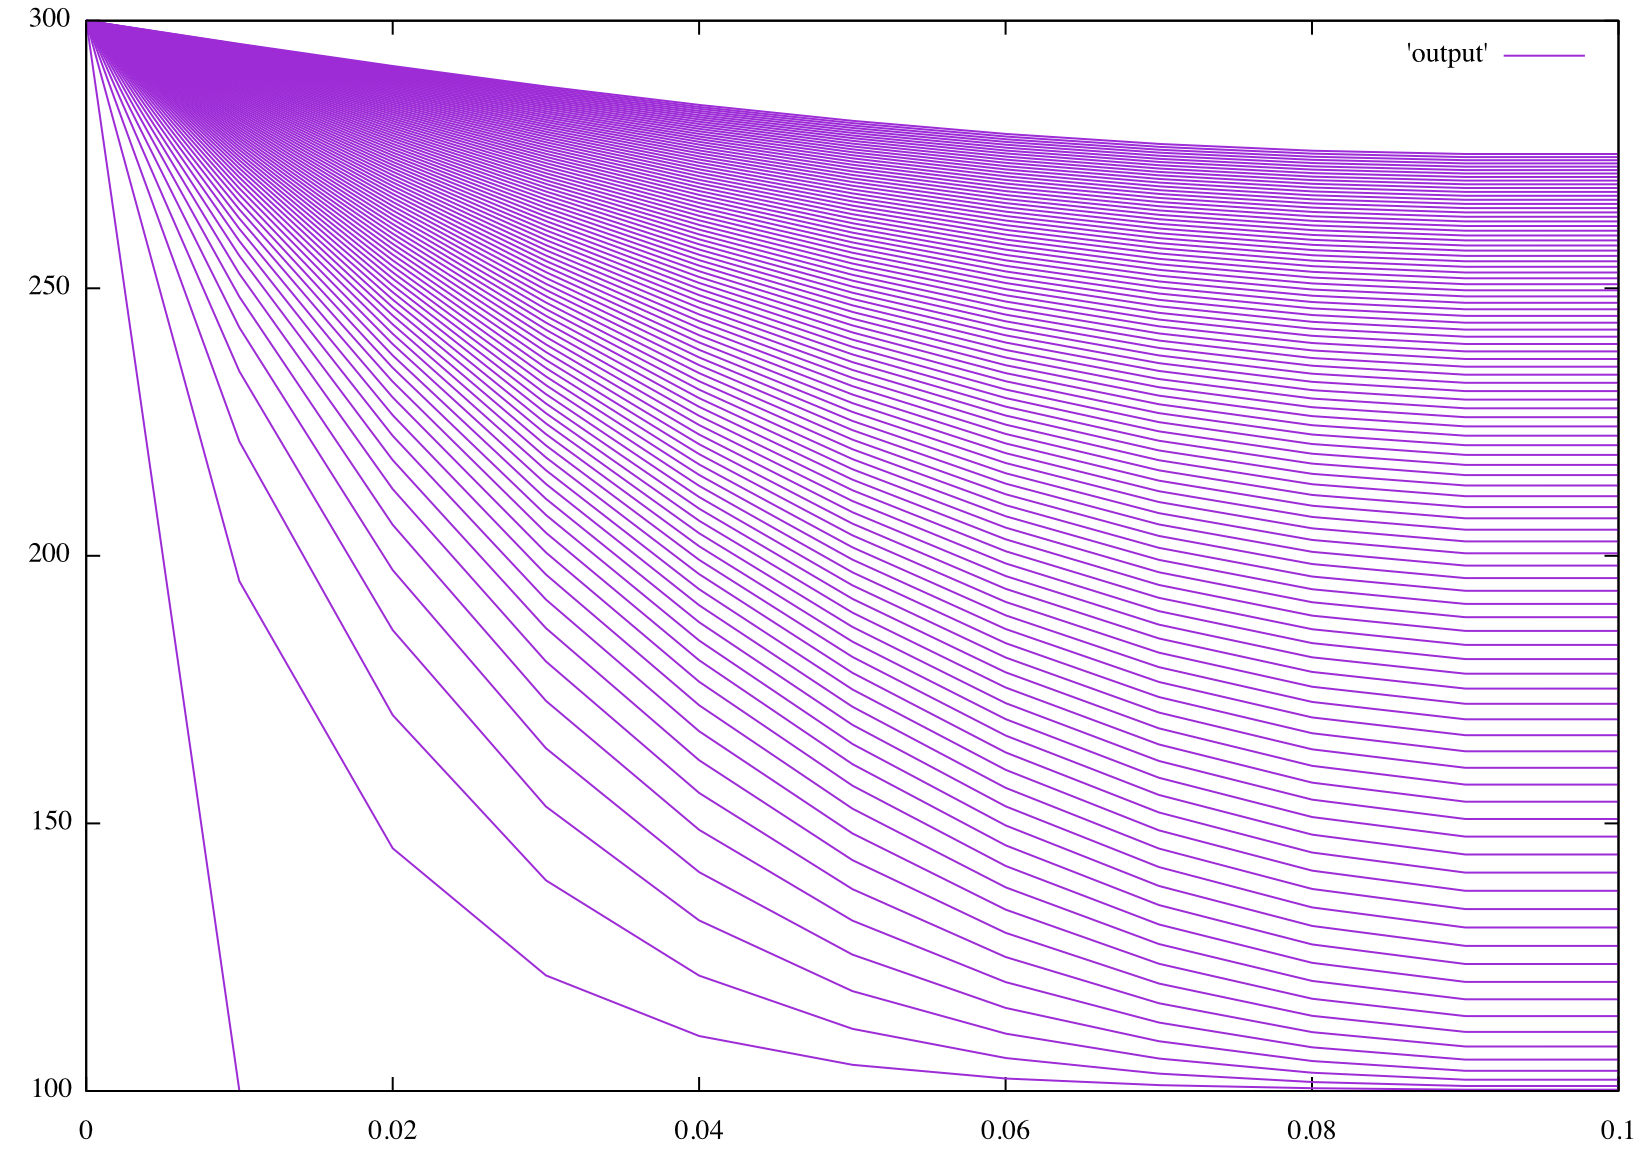
\includegraphics[width=100mm]{heat.png}
	\end{center}
\end{figure}

\section{実践的な解法}
後退差分による差分近似式を$T_{i,j+1}$について整理すると次式になる。
\begin{equation}
T_{i,j+1}=\frac{T_{i,j}+\alpha \gamma (T_{i+1,j+1} + T_{i-1,j+1})}{1+2 \alpha \gamma}
\end{equation}
上式を線形反復式として解くこともできる。この場合は行列を意識することがなく簡潔になる。
プログラム例は以下になり、同様の結果を得ることができる。
\verbatimtabinput{heat_gs_p.py}
\end{document}